\section{API and Protocol Specification}
\label{sec:api}

Five channels carry everything in this system, and \cref{sec:protocols} said which runs where
and why. This section specifies what travels on each one.

\subsection{HTTP: browser to back office}
\label{sec:api-http}

Nine servlets, mapped with \texttt{@WebServlet} annotations.
Everything is rendered server-side and forwarded to a JSP; there is no JSON API on this
channel, because the browser receives pages.

\begin{table}[h]
\centering\small
\renewcommand{\arraystretch}{1.15}
\caption{HTTP endpoints of the back office. The last column marks the ones behind
\texttt{AuthFilter}.}
\label{tab:http}
\begin{tabularx}{\textwidth}{@{}l l X c@{}}
\toprule
Path & Method & Effect & Auth \\
\midrule
\texttt{/register} & POST & creates the account and its vehicle profile & \\
\texttt{/login} & POST & authenticates, opens the \texttt{HttpSession}, mints the JWT & \\
\texttt{/logout} & GET & invalidates the session & \\
\texttt{/stations} & GET & the directory, read from \texttt{StationDirectory} in memory &
  $\bullet$ \\
\texttt{/station} & GET & one station's page, with the JWT and the WebSocket URL &
  $\bullet$ \\
\texttt{/session} & GET & the live session page for a connector & $\bullet$ \\
\texttt{/profile} & GET & account and vehicle & $\bullet$ \\
\texttt{/history} & GET & past sessions with their invoices & $\bullet$ \\
\texttt{/notifications} & GET & notifications stored for this driver & $\bullet$ \\
\bottomrule
\end{tabularx}
\end{table}

\subsubsection{The token the station will trust}
\label{sec:api-jwt}

A station has to recognise a driver without asking the back office, which is what keeps a
site working while Tomcat is down. The token is the only thing the two sides share.

It is a JWT signed with \textbf{HS256} using a symmetric secret, passed to both sides in the
environment as \texttt{VOLTSHARE\_JWT\_SECRET}. It lives 60 minutes. Java signs with \texttt{jjwt},
Erlang verifies with \texttt{jose}.

\begin{lstlisting}[language=json, caption={The claims, plus the standard \texttt{iat}.},
                   label={lst:jwt}]
{ "sub": "12", "username": "andrea", "vehicle_id": 88,
  "iss": "voltshare-backoffice", "exp": 1755792000 }
\end{lstlisting}

\texttt{sub} is the user id as a string, which the JWT specification requires, and
\texttt{vehicle\_id} is a number. The station needs both: the first attributes the session
to an account, the second matches the claim, which is per vehicle.

On the first frame of the WebSocket the station verifies the signature, checks that \texttt{iss} is exactly
\texttt{voltshare-backoffice}, checks that \texttt{exp} is in the future, and extracts the
two identifiers. A failure closes the socket with \texttt{4401}, an expired token with
\texttt{4408}. The station never calls the back office about a token, whether it accepts one
or throws it out.

There is a trap here that the library invites, and \texttt{contracts/sample-tokens.md}
records it: \texttt{jose\_jwt:verify/2} checks \emph{only the signature}. Issuer and expiry
are ordinary claims, so a token that verifies is not yet a token to accept, and both checks
are written out explicitly on the station side.

\paragraph{How the token reaches the browser.} The servlet puts it in the session, the JSP
renders it into a hidden \texttt{data-} attribute through \texttt{<c:out>}, and the
WebSocket code reads it from there. 

\subsection{WebSocket: driver to station}
\label{sec:api-ws-driver}

The page opens \texttt{ws://<station>:8080/ws/driver?station\_id=<id>}. Host and port are
what the station announced about itself, republished by \texttt{StationDirectory}
(\cref{sec:api-bridge}). The page appends the query string, naming the station it believes
it is showing. A mismatch closes the socket with \texttt{4400}.

Frames are text, one JSON object each, and both directions share one envelope.

\begin{lstlisting}[language=json, label={lst:envelope},
  caption={The envelope of both WebSocket channels. A \texttt{payload} is \texttt{\{\}} when
  there is nothing to say.}]
// browser -> station
{ "action": "reserve", "request_id": "3f2c9a",
  "payload": { "connector_id": 3 } }

// station -> browser
{ "type": "ack", "request_id": "3f2c9a",
  "payload": { "expires_at": 1757250000000, "lease_seconds": 900 } }
\end{lstlisting}

Every decision is taken in \texttt{vs\_driver\_proto}, a module of pure functions over a
session map, so the whole contract runs under EUnit with no listener.
\texttt{vs\_driver\_ws} holds the Cowboy callbacks and nothing else. The rest of this
subsection walks the channel in the order the frames occur, with the real shape of each one.

\paragraph{Join, and nothing before it.} The socket starts unauthenticated, and the first
frame has to be a \texttt{join} carrying the JWT of \cref{sec:api-jwt}, within 5~s.

\begin{lstlisting}[style=msg]
{ "action": "join", "request_id": "r-join",
  "payload": { "token": "eyJhbGciOiJIUzI1NiJ9.eyJzdWIiOiIxMiIs...<sig>" } }
\end{lstlisting}

\texttt{token} is the only field read. The station verifies it locally and binds
\texttt{user\_id} and \texttt{vehicle\_id} to the connection, so a payload that also carries
a \texttt{user\_id} changes nothing. The answer is an empty \texttt{ack}, with the first
\texttt{state} behind it in the same write.

\begin{lstlisting}[style=msg]
{ "type": "ack", "request_id": "r-join", "payload": {} }
\end{lstlisting}

\paragraph{Reserve, cancel, stop.} Three actions follow, and every one names a connector.

\begin{lstlisting}[style=msg]
{ "action": "reserve", "request_id": "a1", "payload": { "connector_id": 3 } }
\end{lstlisting}

The station asks the coordinator for a claim before it touches the connector
(\cref{sec:api-claim}). Only if the claim is granted does the connector go \texttt{held},
and the \texttt{ack} carries the lease that the page counts down from.

\begin{lstlisting}[style=msg]
{ "type": "ack", "request_id": "a1",
  "payload": { "connector_id": 3,
               "expires_at": 1757250000000, "lease_seconds": 900 } }
\end{lstlisting}

\texttt{expires\_at} is epoch milliseconds and \texttt{lease\_seconds} is the same lease as a
duration, both from the station's clock. A refusal arrives instead, echoing the same
\texttt{request\_id} and carrying a code from \cref{tab:driver-errors}.

\begin{lstlisting}[style=msg]
{ "type": "error", "request_id": "a1",
  "payload": { "code": "ALREADY_HELD",
               "message": "connector 3 is held by another driver" } }
\end{lstlisting}

\texttt{cancel\_reservation} and \texttt{stop\_session} carry the payload of
\texttt{reserve} and are acknowledged with the connector alone,
\texttt{"payload": \{ "connector\_id": 3 \}}. Cancelling frees the connector at once and
releases the claim, with no penalty, which is the whole incentive to cancel. Stopping tells
the charge point to stop and returns the connector's share to the pool, while the session
row waits for the vehicle to be unplugged.

\Cref{fig:seq-reserve} puts these frames on a timeline, with a lost \texttt{ack} and a
second reservation for the same vehicle.

\begin{figure}[t]
\centering
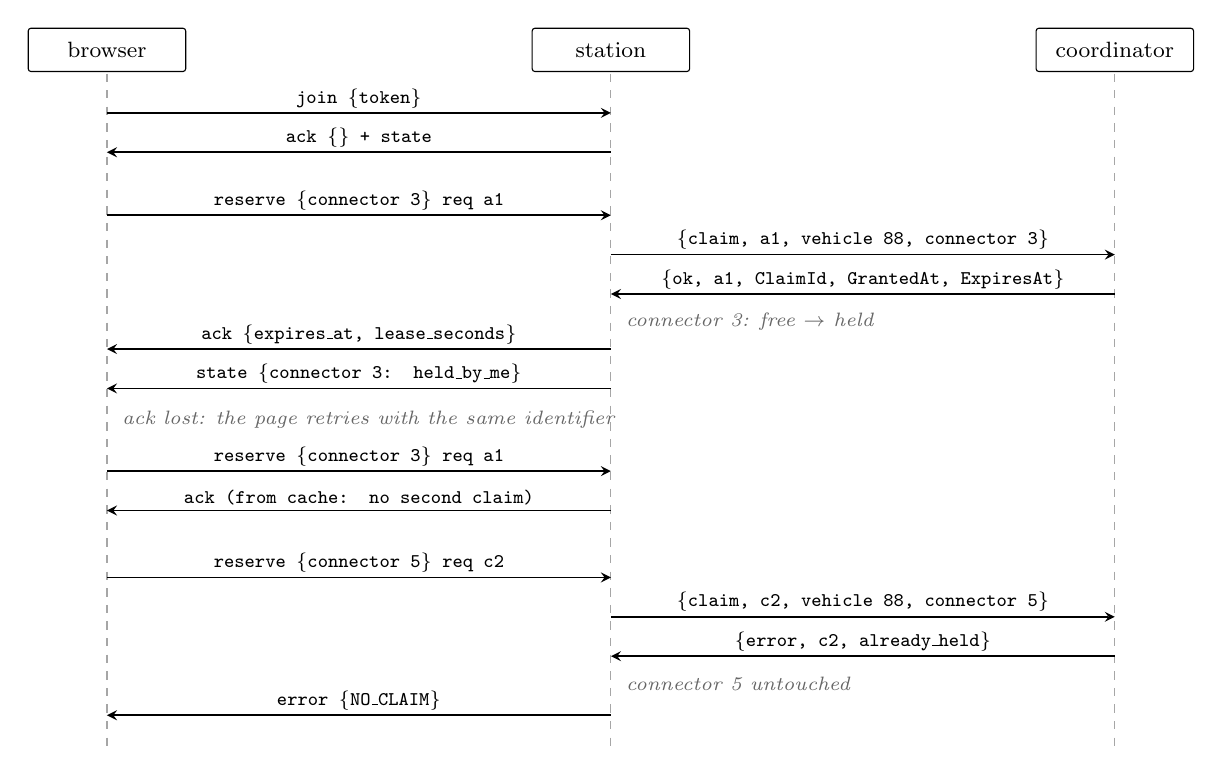
\begin{tikzpicture}[>=stealth, font=\footnotesize, x=1cm, y=1cm,
  msg/.style={->, semithick},
  lab/.style={font=\scriptsize\ttfamily, fill=white, inner sep=1.5pt, midway},
  note/.style={font=\scriptsize\itshape, text=black!60, anchor=west, inner sep=1pt}]
  \foreach \x/\n in {0/browser, 6.4/station, 12.8/coordinator} {
    \node[draw, rounded corners=1pt, minimum width=2cm, minimum height=0.55cm] at (\x,0) {\n};
    \draw[black!35, dashed] (\x,-0.3) -- (\x,-8.9);
  }
  \draw[msg] (0,-0.8) -- (6.4,-0.8) node[lab, above] {join \{token\}};
  \draw[msg] (6.4,-1.3) -- (0,-1.3) node[lab, above] {ack \{\} + state};
  \draw[msg] (0,-2.1) -- (6.4,-2.1) node[lab, above] {reserve \{connector 3\}  req a1};
  \draw[msg] (6.4,-2.6) -- (12.8,-2.6) node[lab, above] {\{claim, a1, vehicle 88, connector 3\}};
  \draw[msg] (12.8,-3.1) -- (6.4,-3.1) node[lab, above] {\{ok, a1, ClaimId, GrantedAt, ExpiresAt\}};
  \node[note] at (6.55,-3.45) {connector 3: free $\rightarrow$ held};
  \draw[msg] (6.4,-3.8) -- (0,-3.8) node[lab, above] {ack \{expires\_at, lease\_seconds\}};
  \draw[msg] (6.4,-4.3) -- (0,-4.3) node[lab, above] {state \{connector 3: held\_by\_me\}};
  \node[note] at (0.15,-4.7) {ack lost: the page retries with the same identifier};
  \draw[msg] (0,-5.35) -- (6.4,-5.35) node[lab, above] {reserve \{connector 3\}  req a1};
  \draw[msg] (6.4,-5.85) -- (0,-5.85) node[lab, above] {ack (from cache: no second claim)};
  \draw[msg] (0,-6.7) -- (6.4,-6.7) node[lab, above] {reserve \{connector 5\}  req c2};
  \draw[msg] (6.4,-7.2) -- (12.8,-7.2) node[lab, above] {\{claim, c2, vehicle 88, connector 5\}};
  \draw[msg] (12.8,-7.7) -- (6.4,-7.7) node[lab, above] {\{error, c2, already\_held\}};
  \node[note] at (6.55,-8.05) {connector 5 untouched};
  \draw[msg] (6.4,-8.45) -- (0,-8.45) node[lab, above] {error \{NO\_CLAIM\}};
\end{tikzpicture}
\caption{A reservation on the driver channel: the claim precedes the commit, a retried
\texttt{reserve} is answered from the cache, and a second reservation for the same vehicle
is refused by the coordinator before the station touches the connector.}
\label{fig:seq-reserve}
\end{figure}

\paragraph{What the station pushes.} \texttt{ack} and \texttt{error} answer an action and
echo its \texttt{request\_id}. The other three arrive unasked and carry \texttt{null} there.
\texttt{state} is the whole station, sent on join, on every change, and every 5~s.

\begin{lstlisting}[style=msg]
{ "type": "state", "request_id": null,
  "payload": {
    "station_id": 1, "name": "Pisa Centro",
    "site_power_kw": 350, "allocated_kw": 210.5, "tariff_cents_kwh": 45,
    "coordinator_reachable": true,
    "connectors": [
      { "connector_id": 2, "state": "held", "rated_kw": 150, "power_kw": 0,
        "held_by_me": true, "mine": true, "expires_at": 1757250000000 },
      { "connector_id": 3, "state": "charging", "rated_kw": 150,
        "held_by_me": false, "mine": false, "expires_at": null,
        "power_kw": 120.0 } ],
    "waitlist": { "length": 0, "my_position": null } } }
\end{lstlisting}

A connector's \texttt{state} is one of \texttt{free}, \texttt{held}, \texttt{charging},
\texttt{suspended}, \texttt{complete}, \texttt{overstay}, \texttt{closing} and
\texttt{out\_of\_service}, the last being the wire name for a connector with no process
answering for it. \texttt{held\_by\_me} and \texttt{mine} are not synonyms: the first means
the reservation belongs to this driver, the second also covers a session in progress. The
\texttt{waitlist} object is a constant, left in place for the feature of \cref{sec:future}.
The periodic tick earns its place beside the event-driven pushes, because meter readings
change \texttt{power\_kw} without raising a connector event, and an event-only channel would
show a live session at a frozen power. A WebSocket \texttt{ping} rides on the same tick, so
that Cowboy's inbound-only idle timeout does not hang up on a page that is only watching.

\texttt{session} goes out with each \texttt{state}, and only to the owner of a running
session. A driver without one gets no frame at all, instead of a frame of zeros.

\begin{lstlisting}[style=msg]
{ "type": "session", "request_id": null,
  "payload": { "connector_id": 2, "phase": "charging",
               "power_kw": 89.4, "energy_kwh": 12.317, "soc_pct": 58,
               "eta_seconds": 981, "started_at": 1757248000000,
               "overstay_seconds": 0 } }
\end{lstlisting}

\texttt{phase} is \texttt{charging}, \texttt{suspended}, \texttt{complete},
\texttt{overstay} or \texttt{closed}, read off the connector in that order of precedence, so
that a car which is both full and past its grace period reports \texttt{overstay}.
\texttt{eta\_seconds} is \texttt{null} while nothing is being delivered.
\texttt{overstay\_seconds} is already net of the grace, and it is the same number that ends
up in \texttt{sessions.\allowbreak overstay\_seconds}. A session ends by disappearing from
the snapshot, and that disappearance becomes one last frame with the phase \texttt{closed}.

\begin{lstlisting}[style=msg]
{ "type": "notification", "request_id": null,
  "payload": { "kind": "reservation_expiring", "connector_id": 3,
      "text": "Your reservation expires in less than two minutes." } }
\end{lstlisting}

There are six kinds: \texttt{reservation\_expiring}, \texttt{reservation\_expired},
\texttt{claim\_revoked}, \texttt{charge\_complete}, \texttt{overstay\_started} and
\texttt{session\_interrupted}. The manager broadcasts each event to every subscribed socket,
and a socket delivers it only when the user it names is the user its token bound. One table
supplies the sentence for this frame and for the durable copy that reaches
\texttt{notifications.jsp}, so both say the same words.

\paragraph{Two ways for something to go wrong.} A refused action produces an \texttt{error}
frame and leaves the connection open. \Cref{tab:driver-errors} is the whole set of nine
codes, and a driver waiting on a reservation always gets one of them or an \texttt{ack}.

\begin{table}[h]
\centering\small
\renewcommand{\arraystretch}{1.15}
\caption{The nine application error codes, carried in the \texttt{code} field of an
\texttt{error} frame. The \texttt{message} beside them is written for the driver and the
page shows it verbatim.}
\label{tab:driver-errors}
\begin{tabularx}{\textwidth}{@{}l X@{}}
\toprule
Code & Raised when \\
\midrule
\texttt{BAD\_REQUEST} & the frame is unusable: no \texttt{request\_id}, no \texttt{payload}
  object, an unknown action, or a \texttt{connector\_id} that is not a positive integer \\
\texttt{UNAUTHENTICATED} & an action arrived before \texttt{join} succeeded, and the socket
  is then closed with \texttt{4401} \\
\texttt{UNKNOWN\_CONNECTOR} & that connector is not one of this station's \\
\texttt{RETRY\_LATER} & the condition is temporary: the coordinator is rebuilding, the
  station is starting, or the connector process is between a crash and its restart \\
\texttt{ALREADY\_HELD} & another driver holds that connector \\
\texttt{NO\_CLAIM} & the vehicle already holds a reservation, or the coordinator never
  answered \\
\texttt{SUSPENDED} & the account is serving a no-show penalty, and walk-in charging still
  works \\
\texttt{NOT\_YOURS} & that reservation or session belongs to another account \\
\texttt{INVALID\_STATE} & the action does not apply to the connector as it is now \\
\bottomrule
\end{tabularx}
\end{table}

A close code is the other kind, and it ends the connection. \texttt{4400} covers a binary
frame, malformed JSON or a wrong \texttt{station\_id}. \texttt{4401} covers a bad token, an
action before \texttt{join}, or no \texttt{join} within the 5~s. \texttt{4408} is an expired
token, kept apart so that the page can tell ``log in again'' from ``something is wrong''.
\texttt{1001} is the station shutting down. The page treats the first three as final and
answers the last by reconnecting with backoff.

\paragraph{Decisions on this channel.}
\begin{itemize}
  \item \textbf{Identity comes from the token alone.} \texttt{held\_by\_me}
        and \texttt{mine} are computed on the station. A notification is delivered only when
        the user it names is the one the token bound, a filter written as a pattern in the
        clause head of \texttt{websocket\_info/2}. The alternative was a \texttt{user\_id}
        field in the request. It would let a driver reserve or cancel for somebody else by
        editing a frame.
  \item \textbf{One \texttt{RETRY\_LATER}, with the cause in the message.} Three facts share
        the code: the coordinator is rebuilding, the station is starting, or the connector
        process is between a crash and its restart. The client does the same thing in all
        three. Three codes would put a piece of the station's internals into every client.
        The third case used to be answered \texttt{UNKNOWN\_CONNECTOR}, a permanent code for
        a condition that lasts milliseconds.
  \item \textbf{The socket keeps no state; the connector process does.} Reconnection is the
        client's job: backoff from 500~ms, capped at 10~s, then a fresh \texttt{join}. The
        station keeps nothing for a disconnected socket. The reservation lives in the
        connector process and survives the browser being closed.
\end{itemize}

\subsection{WebSocket: charge point to station}
\label{sec:api-ws-cp}

This channel is the boundary of the system. Above it is production logic, below it is
emulated hardware. The emulator is credible only if a real charge point could implement the
same interface. The message set is a reduced OCPP 1.6-J~\cite{ocpp16j}: the same direction
of authority, a fraction of the surface. \Cref{tab:cp-messages} maps every message to its
original.

The charge point is the client. It dials
\texttt{ws://<station>:8081/\allowbreak ws/cp?\allowbreak station\_id=<id>\allowbreak
\&connector\_id=<n>} the way real equipment dials an operator's backend from behind the
NAT of a site network. The envelope is the one of \cref{lst:envelope}, so one codec serves
both channels, but here \texttt{request\_id} is only a correlation key for the logs. Nothing
is retried on this channel and there are no \texttt{error} frames, so a frame the station
cannot read is logged and dropped. There is no authentication either. The link is
site-local. A real deployment would use mutual TLS, which we did not implement.

\begin{table}[h]
\centering\small
\renewcommand{\arraystretch}{1.15}
\caption{The message set, and the OCPP 1.6-J message each one reduces. Four OCPP
operations (\texttt{DataTransfer}, \texttt{FirmwareUpdate}, \texttt{Reset},
\texttt{UnlockConnector}) have no counterpart: they belong to operations, which this
system does not model.}
\label{tab:cp-messages}
\begin{tabularx}{\textwidth}{@{}l l >{\raggedright\arraybackslash}p{3.9cm} X@{}}
\toprule
Message & Dir. & OCPP 1.6-J & Payload and effect \\
\midrule
\texttt{boot} & $\to$ & \texttt{BootNotification} & vendor, model, firmware,
  \texttt{rated\_kw}, physical \texttt{status}; binds the socket to the connector \\
\texttt{heartbeat} & $\to$ & \texttt{Heartbeat} & empty; the \texttt{ack} returns
  \texttt{server\_time} \\
\texttt{status} & $\to$ & \texttt{StatusNotification} & \texttt{available},
  \texttt{occupied}, \texttt{faulted}, \texttt{unavailable}: nine OCPP states reduced to four,
  no error taxonomy \\
\texttt{plugged} & $\to$ & \texttt{Authorize} + \texttt{StartTransaction} &
  \texttt{vehicle\_id}, \texttt{soc\_pct}, \texttt{battery\_kwh}, \texttt{max\_kw}; id tags and
  the local authorisation cache are dropped \\
\texttt{meter} & $\to$ & \texttt{MeterValues} & \texttt{power\_kw}, cumulative
  \texttt{energy\_kwh}, \texttt{soc\_pct}: three measurands out of the sampled-value matrix \\
\texttt{unplugged} & $\to$ & \texttt{StopTransaction} & final \texttt{energy\_kwh}; the
  session row is written here \\
\texttt{set\_limit} & $\leftarrow$ & \texttt{SetChargingProfile} & \texttt{limit\_kw}, a
  single instantaneous ceiling; profiles, schedules and stacking levels are gone \\
\texttt{stop} & $\leftarrow$ & \texttt{RemoteStopTransaction} & \texttt{reason}, one of
  six \\
\bottomrule
\end{tabularx}
\end{table}

\paragraph{Boot.} The handshake is followed by a \texttt{boot}, which is where the socket is
bound to the connector.

\begin{lstlisting}[style=msg]
{ "action": "boot", "request_id": "cp-1",
  "payload": { "vendor": "VoltShare-Emu", "model": "EMU-150", "firmware": "0.1.0",
               "rated_kw": 150, "status": "available" } }
\end{lstlisting}

Only \texttt{status} has an effect. The other four fields end up in one line of the log,
because the rating that governs the allocation is the station's own record of the connector
and not what the equipment claims about itself. The \texttt{ack} carries everything the
equipment needs in order to behave, so the equipment holds no configuration of its own.

\begin{lstlisting}[style=msg]
{ "type": "ack", "request_id": "cp-1",
  "payload": { "accepted": true,
      "heartbeat_interval_s": 30, "meter_interval_s": 5,
      "server_time": 1757248000000, "limit_kw": 60.0 } }
\end{lstlisting}

A connector configured here may have no process behind it at that instant, because the node
is starting or its supervisor is restarting it. The socket is admitted anyway, and the
refusal comes at the \texttt{boot} with the reason in words. \texttt{connector not ready} is
temporary and the equipment retries on its own backoff, while \texttt{unknown connector} is
permanent and the next handshake will be closed outright.

\begin{lstlisting}[style=msg]
{ "type": "ack", "request_id": "cp-1",
  "payload": { "accepted": false, "reason": "connector not ready" } }
\end{lstlisting}

\paragraph{Heartbeat and status.} A \texttt{heartbeat} every 30~s, with an empty payload,
answered with the station's clock. It is the only other message that gets an \texttt{ack};
\texttt{status}, \texttt{plugged}, \texttt{meter} and \texttt{unplugged} get none.

\begin{lstlisting}[style=msg]
{ "action": "heartbeat", "request_id": "cp-42", "payload": {} }
{ "type": "ack", "request_id": "cp-42",
  "payload": { "server_time": 1757248000000 } }

{ "action": "status", "request_id": "cp-7", "payload": { "status": "available" } }
\end{lstlisting}

The four \texttt{status} values are \texttt{available}, \texttt{occupied},
\texttt{faulted} and \texttt{unavailable}. Anything else is logged as unusable and dropped,
without creating an atom, so a talkative or broken charge point cannot grow the atom table.

\paragraph{Plugged.} This is where authorisation happens, and nowhere else.

\begin{lstlisting}[style=msg]
{ "action": "plugged", "request_id": "cp-8",
  "payload": { "vehicle_id": 88, "soc_pct": 22,
      "battery_kwh": 58, "max_kw": 150 } }
\end{lstlisting}

The payload names a vehicle, and the station resolves it to an account locally. That lookup
is the one an isolated station cannot make (\cref{sec:station-failures}). Two fields decide
whether a session opens at all. Without \texttt{vehicle\_id} there is nobody to bill, and
without \texttt{max\_kw} the allocator of \cref{sec:p5} would compute a demand of zero and
leave the car at zero kilowatts for ever with nothing in any log to say why, so both are
refused rather than defaulted. \texttt{soc\_pct} and \texttt{battery\_kwh} only sharpen the
estimated time of arrival. What the station does next depends on the connector.

\begin{table}[h]
\centering\small
\renewcommand{\arraystretch}{1.15}
\caption{What a \texttt{plugged} does, by connector state.}
\label{tab:plugged}
\begin{tabularx}{\textwidth}{@{}l l X@{}}
\toprule
Connector & Vehicle & Outcome \\
\midrule
\texttt{held} & the reserved one & session starts, lease cancelled, claim kept to the end \\
\texttt{held} & another & \texttt{stop} with \texttt{not\_your\_reservation}; the
  reservation stays \\
\texttt{free} & any & walk-in: session on that vehicle's account, no claim needed \\
\texttt{free} & of a suspended account & session starts anyway: the penalty covers
  reservations only \\
\texttt{charging}, \texttt{complete}, \texttt{closing} & any & refused with no frame;
  physical and logical state have diverged, and the log says so \\
\bottomrule
\end{tabularx}
\end{table}

\paragraph{Meter, commands, unplugged.} While the car draws, a reading every 5~s.

\begin{lstlisting}[style=msg]
{ "action": "meter", "request_id": "cp-9",
  "payload": { "power_kw": 89.4, "energy_kwh": 12.317, "soc_pct": 58 } }
\end{lstlisting}

\texttt{energy\_kwh} is cumulative since the session started. The connector stores
\texttt{max(stored, reported)}, so a counter that resets on a firmware glitch cannot
subtract energy already billed. A \texttt{meter} for a connector with no session is dropped
and logged. The two commands travel the other way, and both carry a \texttt{null}
\texttt{request\_id} because the station starts them.

\begin{lstlisting}[style=msg]
{ "type": "command", "request_id": null,
  "payload": { "command": "set_limit", "limit_kw": 60.0 } }

{ "type": "command", "request_id": null,
  "payload": { "command": "stop", "reason": "station_shutdown" } }
\end{lstlisting}

\texttt{set\_limit} is the allocator's output, and \texttt{limit\_kw: 0.0} means suspended
rather than finished: the session stays open and draws nothing. The six stop reasons are
\texttt{driver\_stopped}, \texttt{target\_reached}, \texttt{claim\_revoked},
\texttt{not\_your\_reservation}, \texttt{faulted} and \texttt{station\_shutdown}. The last
is written by \texttt{vs\_cp\_ws} just before the \texttt{1001} close, because after the
listener is gone there is nobody left to tell. A \texttt{stop} ends the delivery and the
connector stays occupied until the cable comes out, which is what makes an overstay
billable. \texttt{faulted} is the exception: the session is closed at once with the energy
last measured, because faulted equipment may never send another frame.

\begin{lstlisting}[style=msg]
{ "action": "unplugged", "request_id": "cp-10",
  "payload": { "energy_kwh": 41.203 } }
\end{lstlisting}

At that point the station writes the \texttt{sessions} row with energy and overstay,
releases the claim, and moves the connector to \texttt{free}.

\paragraph{Silence.} The contract obliges the equipment to speak, so Cowboy's inbound-only
idle timeout \emph{is} the missed-heartbeat rule and this channel needs no \texttt{ping}.
The budget is three heartbeats, 90~s, and the part worth knowing is that it is spent in
series and not in parallel. Cowboy waits 60~s, two intervals, and closes the socket. Only
then does the connector see the socket die and arm its own 30~s of grace. Adding the two
gives the 90~s. An earlier version had both timers computing the whole budget, and a mute
charge point stayed reservable for three minutes.

\paragraph{Four ways the socket closes.} \texttt{4404} is the permanent one, decided at the
handshake: the query string is unreadable, or it names another station, or the connector is
not one this station owns. \texttt{4409} goes to the socket that is being replaced when a
second one boots for the same connector, and the eviction happens at the \texttt{boot}
rather than at the handshake, so that a half-open connection cannot throw out a working
charge point before saying a word. \texttt{1001} is the station shutting down, written after
the \texttt{stop} frame in the same batch. \texttt{1012}, Service Restart, is the connector
process dying under a socket that is perfectly healthy: the socket monitors the connector,
retries the attachment five times at 500~ms, replays the last \texttt{status} and
\texttt{plugged}, and gives up only after that.

\paragraph{Reconciliation after a station restart.} The connector processes die with the
node, so the station has no memory of the session. The charge point reconnects, boots, and
re-sends \texttt{plugged} with two optional fields.

\begin{lstlisting}[style=msg]
{ "action": "plugged", "request_id": "cp-8",
  "payload": { "vehicle_id": 88, "soc_pct": 58, "battery_kwh": 58, "max_kw": 150,
               "energy_kwh": 12.042, "charging_seconds": 3600 } }
\end{lstlisting}

The station opens a session from those figures instead of stopping a car that is charging
happily. \texttt{started\_at} is \emph{now} minus \texttt{charging\_seconds}, read on the
station's own clock, so two machines whose clocks are minutes apart still produce the same
instant. Before the field existed, on 28 August, a session that crossed two restarts was
written as 12.042~kWh in twenty-three seconds. Measured on 3 September with
\texttt{docker kill station2}: 34.795~kWh before the kill, 34.812 after the restart, and no
row for the session that was lost. The reservation is not reconstructed. In the mirror case,
where the socket survives and only the connector process died, the replay drops
\texttt{charging\_seconds} on purpose, because a duration ages while the copy sits still in
the socket, and refreshes the energy from the last \texttt{meter} instead.

\paragraph{Decisions on this channel.}
\begin{itemize}
  \item \textbf{A subset of OCPP 1.6-J, with the same direction of authority.} Full OCPP
        was rejected for its surface: configuration keys, id tags, a nine-state model,
        charging profiles with stacking levels. The coordination problem needs none of it.
        An invented protocol was rejected too, because it would have left the emulator with
        nothing to be an emulator of. \Cref{tab:cp-messages} is the reduction, message by
        message.
  \item \textbf{Limits are repeated on every tick}, even when unchanged, so a missed frame
        is corrected within one tick. Delta tracking was rejected on a channel with no
        ordering problem to justify it.
  \item \textbf{Timestamps that matter are the station's.} The equipment sends quantities
        it measured itself: cumulative energy and a duration, never an instant. A
        \texttt{started\_at} from the hardware was rejected, because two clocks minutes
        apart would produce two different sessions from one charge.
\end{itemize}

\subsection{Claims: station to coordinator}
\label{sec:api-claim}

Distributed Erlang, with the coordinator a \texttt{gen\_server} registered locally as
\texttt{vs\_coord\_srv} on each coordinator node and addressed as
\texttt{\{vs\_coord\_srv, Node\}}. Calls carry a 2000~ms timeout, and a timeout is treated like an unreachable node.

\begin{table}[h]
\centering\small
\renewcommand{\arraystretch}{1.15}
\caption{The claim protocol. \texttt{ReqId} is generated by the station and echoed back.}
\label{tab:claim}
\begin{tabularx}{\textwidth}{@{}>{\raggedright\arraybackslash}p{3.3cm} l X@{}}
\toprule
Message & Direction & Purpose \\
\midrule
\texttt{claim} & station $\to$ coord & ask before committing a reservation \\
\texttt{renew} & station $\to$ coord & re-present every claim held, every 10~s \\
\texttt{release} & station $\to$ coord & fire and forget, on cancel, expiry or completion \\
\texttt{who\_do\_you\_hold} & coord $\to$ station & the rebuild query of \cref{sec:rebuild} \\
\texttt{station\_up} & station $\to$ coord & announcement, at start-up and every 30~s \\
\texttt{station\_stats} & station $\to$ coord & free, held and charging counters \\
\texttt{session\_closed} & station $\to$ coord & a session row was written, relay it to Java \\
\bottomrule
\end{tabularx}
\end{table}

\subsubsection{Acquire claim}

\begin{lstlisting}[language=Erlang, caption={Request and the four possible replies.},
                   label={lst:claim}]
{claim, ReqId, VehicleId, UserId, StationId, ConnId}

{ok, ReqId, ClaimId, GrantedAt, ExpiresAt}
{error, ReqId, already_held | suspended | rebuilding | unknown_station}
{not_serving, LeaderNode | undefined}
\end{lstlisting}

Each refusal means something different to the driver, so the station maps them apart:
\texttt{already\_held} says this car is committed at another station,
\texttt{suspended} says the account is serving a no-show penalty, and
\texttt{rebuilding} is temporary and produces a retry rather than an error on screen.
\texttt{unknown\_station} means the coordinator has not heard the announcement yet, so the
station re-announces itself and tries once more.

\subsubsection{Renew}

A station renews all its claims in one message every ten seconds. The renewal is what keeps
them alive: a claim is a lease, and one that stops being renewed expires on its own, which
is how a station that dies stops holding vehicles it can no longer serve. The reply names
those still valid and those revoked.

\begin{lstlisting}[language=Erlang]
{renew, StationId, [{ClaimId, VehicleId, ConnId, UserId, GrantedAt}]}
{renewed, Ok, Revoked, NewExpiresAt}
\end{lstlisting}

Every renewal carries \texttt{GrantedAt} and \texttt{UserId}, including the hundredth one
for a claim nothing has disturbed. The reason is recovery: a renewal is how a newly elected
leader learns about claims it never granted. A claim it has never seen is \textbf{accepted} and adopted with the timestamp
the station reports, which is what makes \cref{sec:rebuild} converge even when the rebuild
query reaches nobody.

\subsubsection{Finding the leader}

The station keeps its own record of the current leader in \texttt{vs\_claim\_client}. If the coordinator queried is not the leader, it responds to the station's claim message with a \texttt{not\_serving}. This coordinator replies with the new leader's name if known, and the call is retried once. A \texttt{not\_serving} message lacking this information, a timeout, or a \texttt{noproc} error causes the station to iterate through the configured list using a round-robin approach for up to one full cycle to locate the new leader. This situation can arise following a network partition between coordinators, causing an isolated coordinator to lose track of the current leader.

If the attempt fails, the station gives up and rejects the reservation. It neither queues the request nor blocks the connector management process; this rule ensures that an interruption in the coordination service does not affect vehicles that are already charging.

\subsection{The JInterface bridge: coordinator to back office}
\label{sec:api-bridge}

The back office does not query the cluster but joins it. Java opens an \texttt{OtpNode} named
\texttt{voltshare\_bo}, registers a mailbox called \texttt{backoffice}, and receives Erlang terms
as the coordinator generates them.

Java acts as a \textbf{hidden node}: it participates in the distribution protocol and is addressable
by name.
The bridge runs on its own daemon thread and attempts to reconnect every three seconds;
consequently, restarting the coordinator never requires restarting Tomcat.


\begin{table}[h]
\centering\small
\renewcommand{\arraystretch}{1.15}
\caption{Messages on the bridge.}
\label{tab:bridge}
\begin{tabularx}{\textwidth}{@{}>{\raggedright\arraybackslash}p{3.3cm} l X@{}}
\toprule
Message & Direction & Purpose \\
\midrule
\texttt{stations\_update} & coord $\to$ Java & the complete station list, on change and
  every 30~s \\
\texttt{leader} & coord $\to$ Java & who is serving now \\
\texttt{session\_closed} & coord $\to$ Java & a session was written; price it now \\
\texttt{no\_show}, \texttt{show\_up} & coord $\to$ Java & penalty accounting \\
\texttt{notify} & coord $\to$ Java & something to tell a driver next time they look \\
\texttt{get\_stations} & Java $\to$ coord & asked once on connect, so no page starts empty \\
\texttt{user\_suspended} & Java $\to$ coord & a no-show counter tripped \\
\texttt{user\_unsuspended} & Java $\to$ coord & the penalty expired \\
\bottomrule
\end{tabularx}
\end{table}

\texttt{stations\_update} is always a complete snapshot. \texttt{StationDirectory} replaces
the entire list atomically, as a partial update would leave a station on the page even
after its node had gone offline.

\paragraph{Suspension recovery occurs via push.} The set of suspensions resides in the coordinator's
memory, while the associated counter is stored in MySQL; consequently, a newly started coordinator
has no knowledge of them. Therefore, the back office re-pushes every active suspension upon receiving
each \texttt{leader} announcement. A coordinator that restarts and resumes the role converges
without requiring any explicit request.

Recovery runs in opposite directions on the two edges, and for two reasons. The stations own
the claims and have to be up for the cluster to mean anything, so the leader asks them, and
it cannot serve until they answer: granting without knowing the claims would break P2.
Nobody in the cluster owns a suspension, which lives in the database behind the back office,
and the back office is allowed to be down (\cref{tab:failures}); a leader that had to ask it
would be unable to start serving whenever Tomcat was down. A leader that does not yet know
the suspensions serves anyway, and the only thing it gets wrong is failing to refuse an
account it should have refused, which is why that one can arrive late.


\paragraph{What happens when the bridge fails.} No coordinator reachable at start-up means 
retries every three seconds, and pages that show an empty list with a warning. If a coordinator crashes while Tomcat is running,
the last snapshot remains in memory, marked as obsolete after 90 seconds (i.e., three missed updates). At that point, the warning is issued. If Tomcat dies, the cluster is left in a consistent state, as the back office is responsible for managing the reservations and sessions. Tomcat dying costs the cluster nothing,
and costs nothing durable either. Every message towards the back office is a send to a
mailbox that is no longer there, dropped without an error and without a retry, so the
coordinator neither blocks nor notices; reservations and charging sessions never touch the
back office in the first place. The session rows were written by the stations and are
already in MySQL, so the first sweep after a restart prices everything that closed in the
meantime. What is lost is the notifications raised during the outage, which have no row
behind them.
